\chapter{Importance sampling}

\section{Comparing importance sampling to the \enquote{crude} method}%
\label{ex:031}

\begin{sourcefiles}
  \item[Source code] src/031\_crude\_vs\_importance.c
  \item[Analysis script] src/031\_crude\_vs\_importance.R
  \item[Executable] exe/031\_crude\_vs\_importance
\end{sourcefiles}

The goal was to integrate the function $f(x) = g(x) e^{-x^{2}}$ on $[0,
\infty)$, with $g(x)$ being a slowly varying function. I chose $g(x) = x
\cos x^{2}$, so the exact value of the integral is
\begin{equation}
  \int_{0}^{\infty} f(x) \, dx = \int_{0}^{\infty} x \cos(x^2) e^{-x^{2}}\, dx =
  \dots = \frac{1}{4}.
\end{equation}
Following the suggestion, we multiply and divide by a weighting function defined
as
\begin{equation}
  w(x) = \frac{2}{\sqrt{\pi}} e^{-x^{2}},
\end{equation}
and so we can write
\begin{equation}
  \int_{0}^{\infty} g(x) e^{-x^{2}} \, dx = \frac{\sqrt{\pi}}{2}
  \int_{0}^{\infty} g(x) w(x) \, dx = \frac{\sqrt{\pi}}{2} \int_{0}^{\infty}
  g(x) \, dw(x).
\end{equation}
Therefore, we can sample numbers $x_i$ from $w(x)$ and estimate the integral
with
\begin{equation}
  \int_{0}^{\infty} g(x) e^{-x^{2}} \, dx \approx \frac{\sqrt{\pi}}{2N} \sum_{i
  = 1}^{N} g(x_i).
\end{equation}

To sample from $w(x)$, which is a half-normal distribution with variance $1/2$,
we can use a modified Box-Muller. The idea is to restrict the number generation
to the $x > 0$ half-plane. First, since in this case the variance is not
unitary, we can recompute the cumulative. The marginal distribution over $r$
needs a factor \num{2} in front for normalization, and we obtain
\begin{equation}
  \rho_r(r) = 2re^{-r^{2}} \implies F_r(r) = 1 - e^{-r^{2}} \implies r =
  \sqrt{-\log(1 - u_{1})}, \quad\text{with } u_1 \sim \unif{0}{1}.
\end{equation}
For $\theta$ we sample uniformly over $[-\pi/2, +\pi/2]$ in order to stay in the
$x > 0$ half-plane:
\begin{equation}
  \theta = -\frac{\pi}{2} + \pi u_2, \quad \text{with } u_2 \sim \unif{0}{1}.
\end{equation}
Once we have $r$ and $\theta$ we generate $x$, $y$ distributed according to
$w(x)$ in this way:
\begin{equation}
  x = r \cos\theta,\quad y = r\abs{\sin\theta}.
\end{equation}

In contrast to the importance sampling technique, inside the same C file I also
implemented the \enquote{crude} Monte Carlo integration, that is a simple
average of a set of $f(x_i)$ with $x_i$ sampled uniformly over an interval from
$0$ to a given $x_{\mathrm{max}}$:
\begin{equation}
  \int_{0}^{\infty} g(x) e^{-x^{2}}\, dx \approx \frac{1}{N} \sum_{i = 1}^{N}
  g(x_i) e^{-x_i^2}, \quad \text{with } x_i \sim \unif{0}{x_{\mathrm{max}}}.
\end{equation}
You can see the comparison between the two methods in terms of relative error in
\cref{fig:031}. The importance sampling is definitely more efficient, although
the crude method has a higher variance which can lead to a lower error in lucky
runs. Also, as the number of samples grows the difference between the two
methods shrinks, but this is rather unsurprising.

\begin{figure}
  \centering
  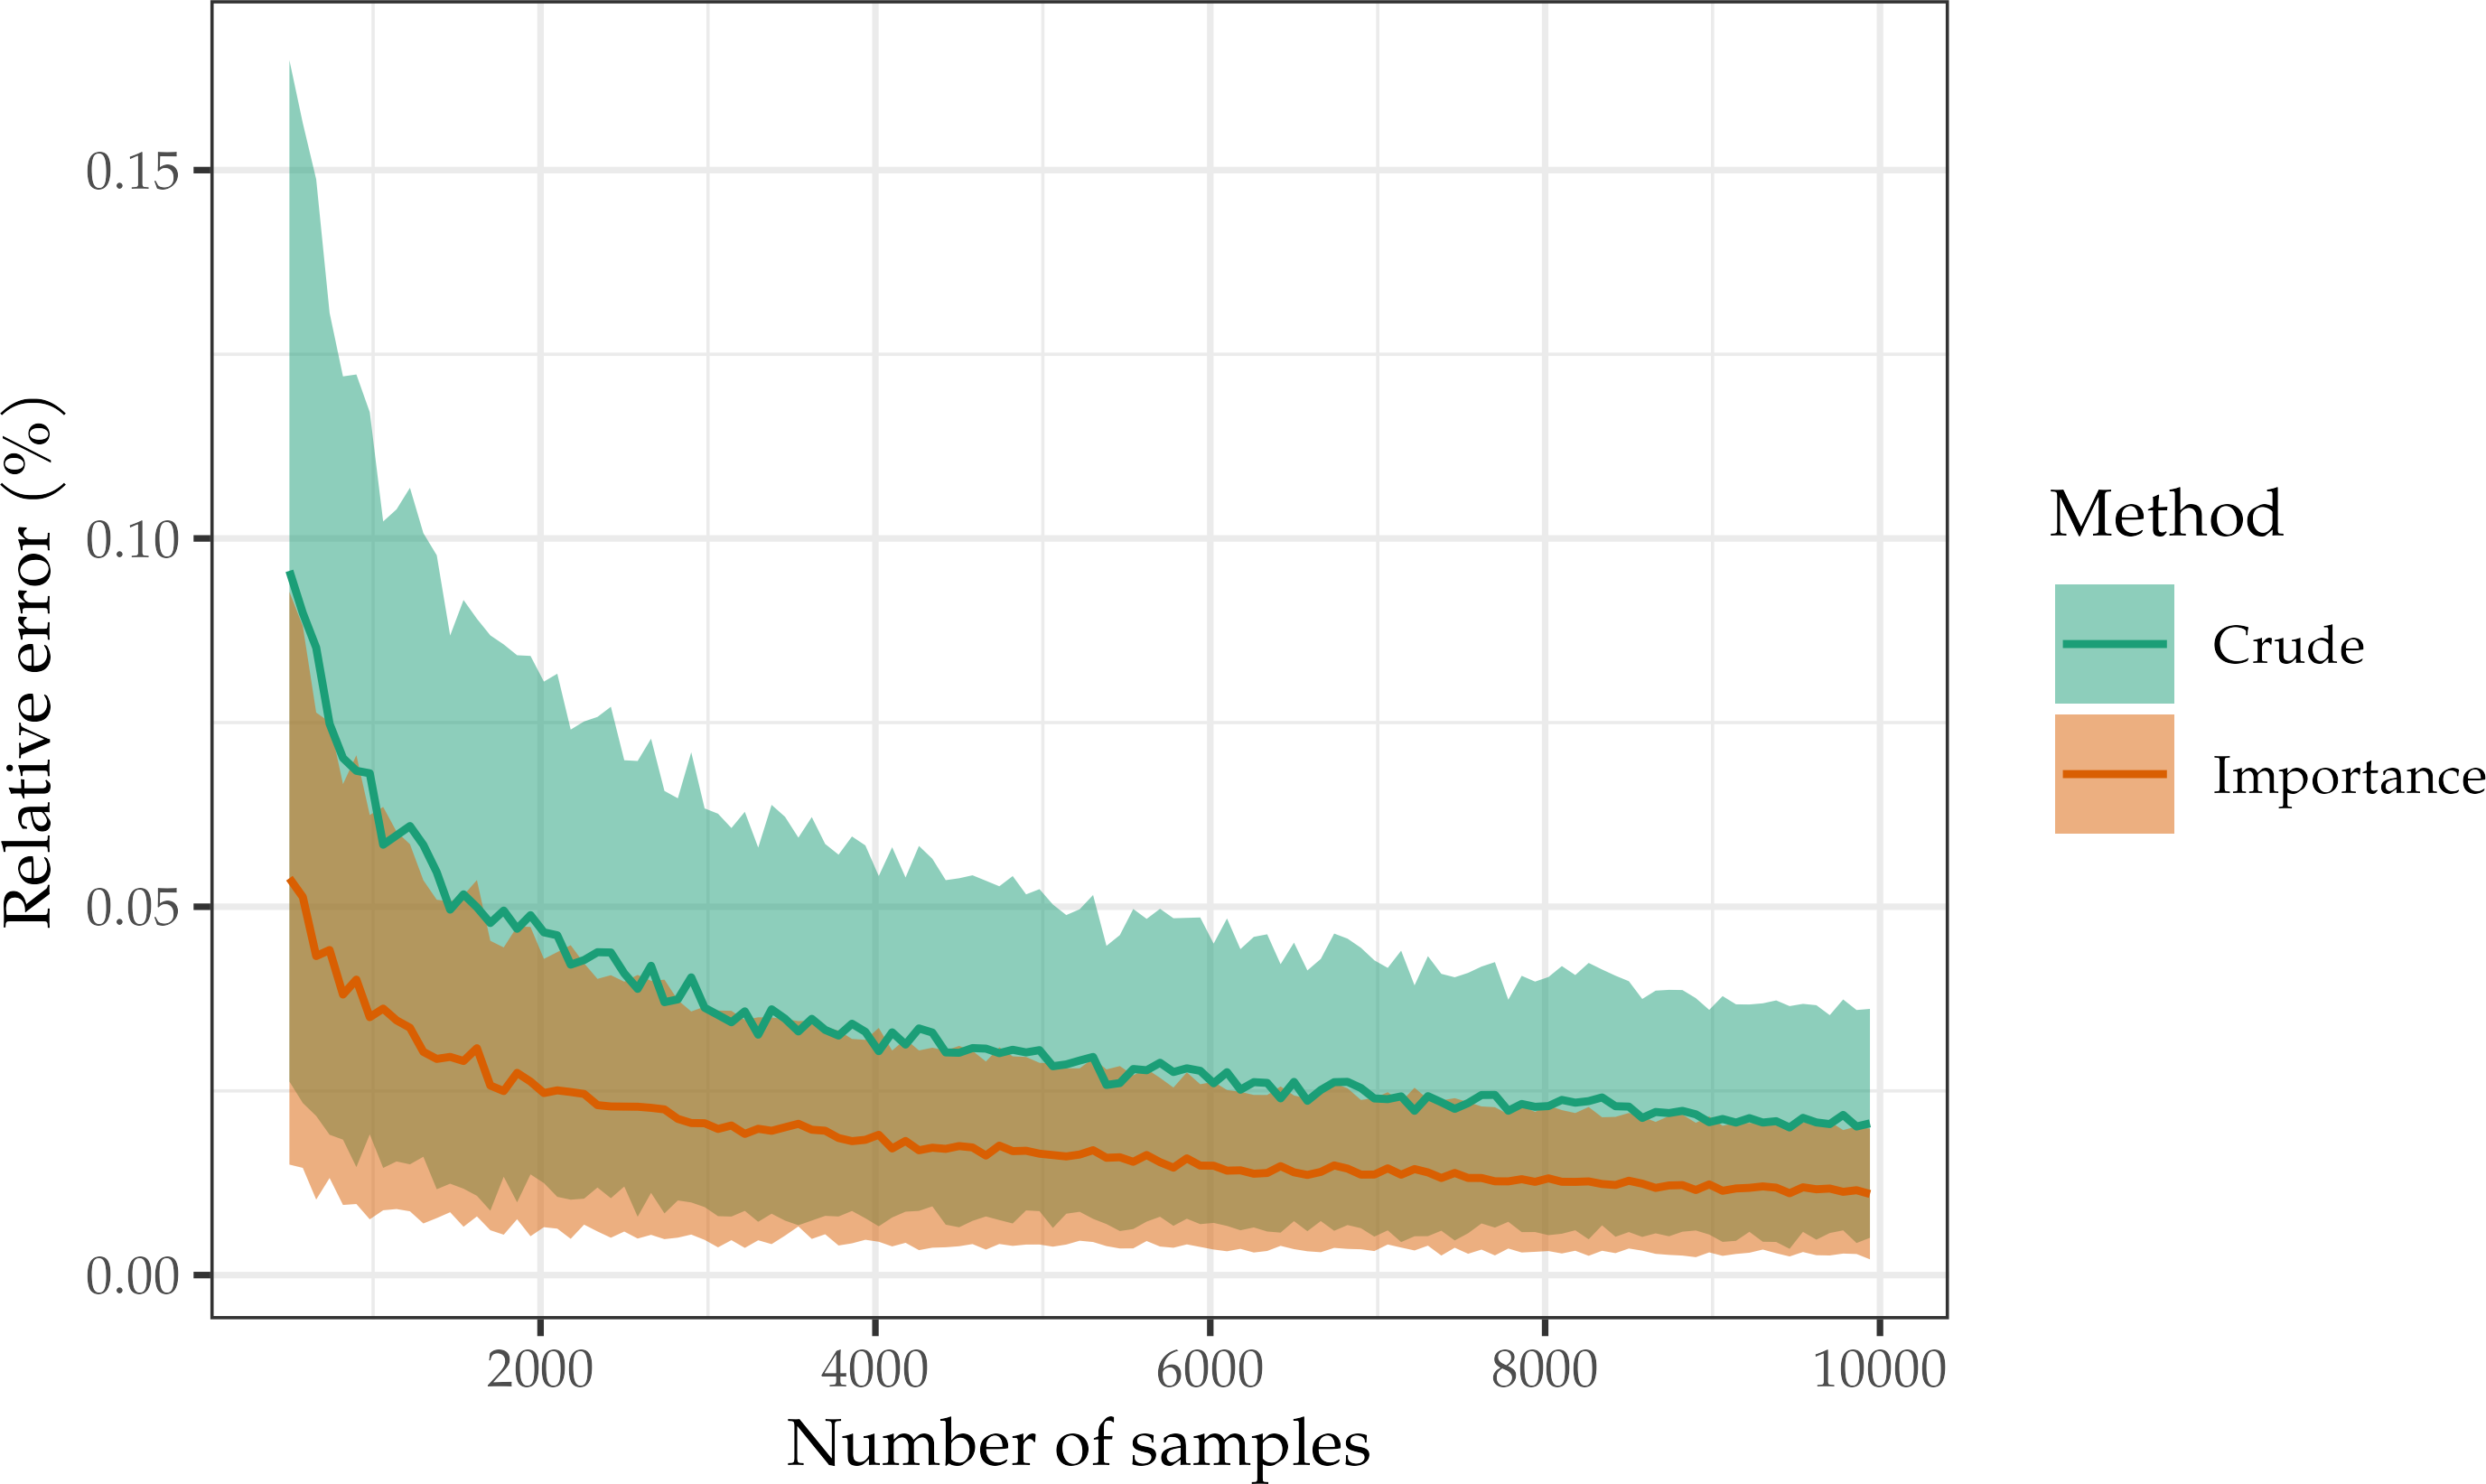
\includegraphics{img/031.png}
  \caption{comparison of the relative error between a \enquote{crude} Monte
    Carlo integration and importance sampling as a function of the number of
    samples. The solid lines represent the average over \num{500} realizations,
    with the standard deviation shaded in the same colour.}
  \label{fig:031}
\end{figure}

\section{Optimizing importance sampling for cosine integration}\label{ex:032}

\begin{sourcefiles}
  \item[Source code] src/032\_cosx\_importance.c
  \item[Analysis script] src/032\_cox\_importance.R
  \item[Executable] exe/032\_cosx\_importance
\end{sourcefiles}

This exercise asked to compute the integral
\begin{equation}
  \int_{0}^{\pi/2} \cos x \, dx
\end{equation}
using once again the importance sampling technique, with a weighting function
$g(x) = a + bx^2$, $a$ and $b$ to tune. To have the best performance, the idea
is to have a $g(x)$ that is large where the integrand is large and small when
the integrand is small. First, $g(x)$ should be normalized, which brings down
the number of parameters to one:
\begin{equation}
  1 = \int_{0}^{\pi/2} (a + bx^{2})\, dx = \frac{\pi}{2}a + \frac{\pi^{3}}{24}b
  \implies a = \frac{2}{\pi} - \frac{\pi^{2}}{12}b.
\end{equation}
Next, since we want $g(x)$ to be as similar as possible to $\cos x$, we can
restrict ourselves to $b < 0$. If $b$ is too negative, though, $g(x)$ becomes
negative in part of the domain. The best solution is to impose $g(\pi/2) = 0$:
\begin{equation}
  0 = \frac{2}{\pi} - \frac{\pi^{2}}{12}b + \frac{\pi^{2}}{4}b \implies b =
  -\frac{12}{\pi^{3}} \implies g(x) = \frac{3}{\pi}\left(1 -
  \frac{4}{\pi^{2}}x^{2}\right).
\end{equation}

To sample from $g$, we compute the cumulative as usual:
\begin{equation}
  G(x) = \frac{3}{\pi} \int_{0}^{x} \left(1 - \frac{4}{\pi^{2}}y^{2}\right)\, dy
  = \frac{3}{\pi}x - \frac{4}{\pi^{3}}x^{3}.
\end{equation}
The inversion requires solving a cubic equation,
\begin{equation}
  u = \frac{3}{\pi} x - \frac{4}{\pi^{3}}x^{3} \implies x^{3} - \frac{3}{4}
  \pi^{2}x + \frac{\pi^{3}}{4} u = 0.
\end{equation}
Let’s define $\alpha = \pi^{2}/4$:
\begin{equation}
  x^{3} - 3\alpha x + \pi \alpha u = 0.
\end{equation}
This is a depressed cubic, so thankfully it has a trigonometric solution given
by\footnote{\url{https://en.wikipedia.org/wiki/Cubic_equation
\#Trigonometric_and_hyperbolic_solutions}.}
\begin{equation}
  x_k = 2 \sqrt{\alpha}
  \cos\left[\frac{1}{3}\arccos\left(-\frac{3\pi\cancel{\alpha}
  u}{6\cancel{\alpha}} \sqrt{\frac{\cancel{3}}{\cancel{3}\alpha}}\right) -
  \frac{2\pi}{3}k \right], \quad \text{with } k = 0, 1, 2.
\end{equation}
With some algebra, and selecting the right $k$, we can arrive at the much simpler form
\begin{equation}
  x = \pi \sin\left(\frac{1}{3} \arcsin u\right), \quad \text{with } u \sim
  \unif{0}{1}.
  \label{eq:xsmp}
\end{equation}

To wrap up, what I ended up doing is
\begin{equation}
  \int_{0}^{\pi/2} \cos x \, dx \approx \frac{1}{N} \sum_{i = 1}^{N} \frac{\cos
  x_{i}}{g(x_{i})} = \frac{\pi}{3N} \sum_{i = 1}^{N} \frac{\cos x_{i}}{1 - 4
  x_{i}^{2} / \pi^{2}},
\end{equation}
with each $x_i$ generated according to \cref{eq:xsmp}. The integration error as
a function of the number of iterations is reported in \cref{fig:032}. Remarkably
as low as \num{100} or \num{200} iterations are sufficient to get, on average,
an error that is comfortably under \qty{1}{\percent}.

\begin{figure}
  \centering
  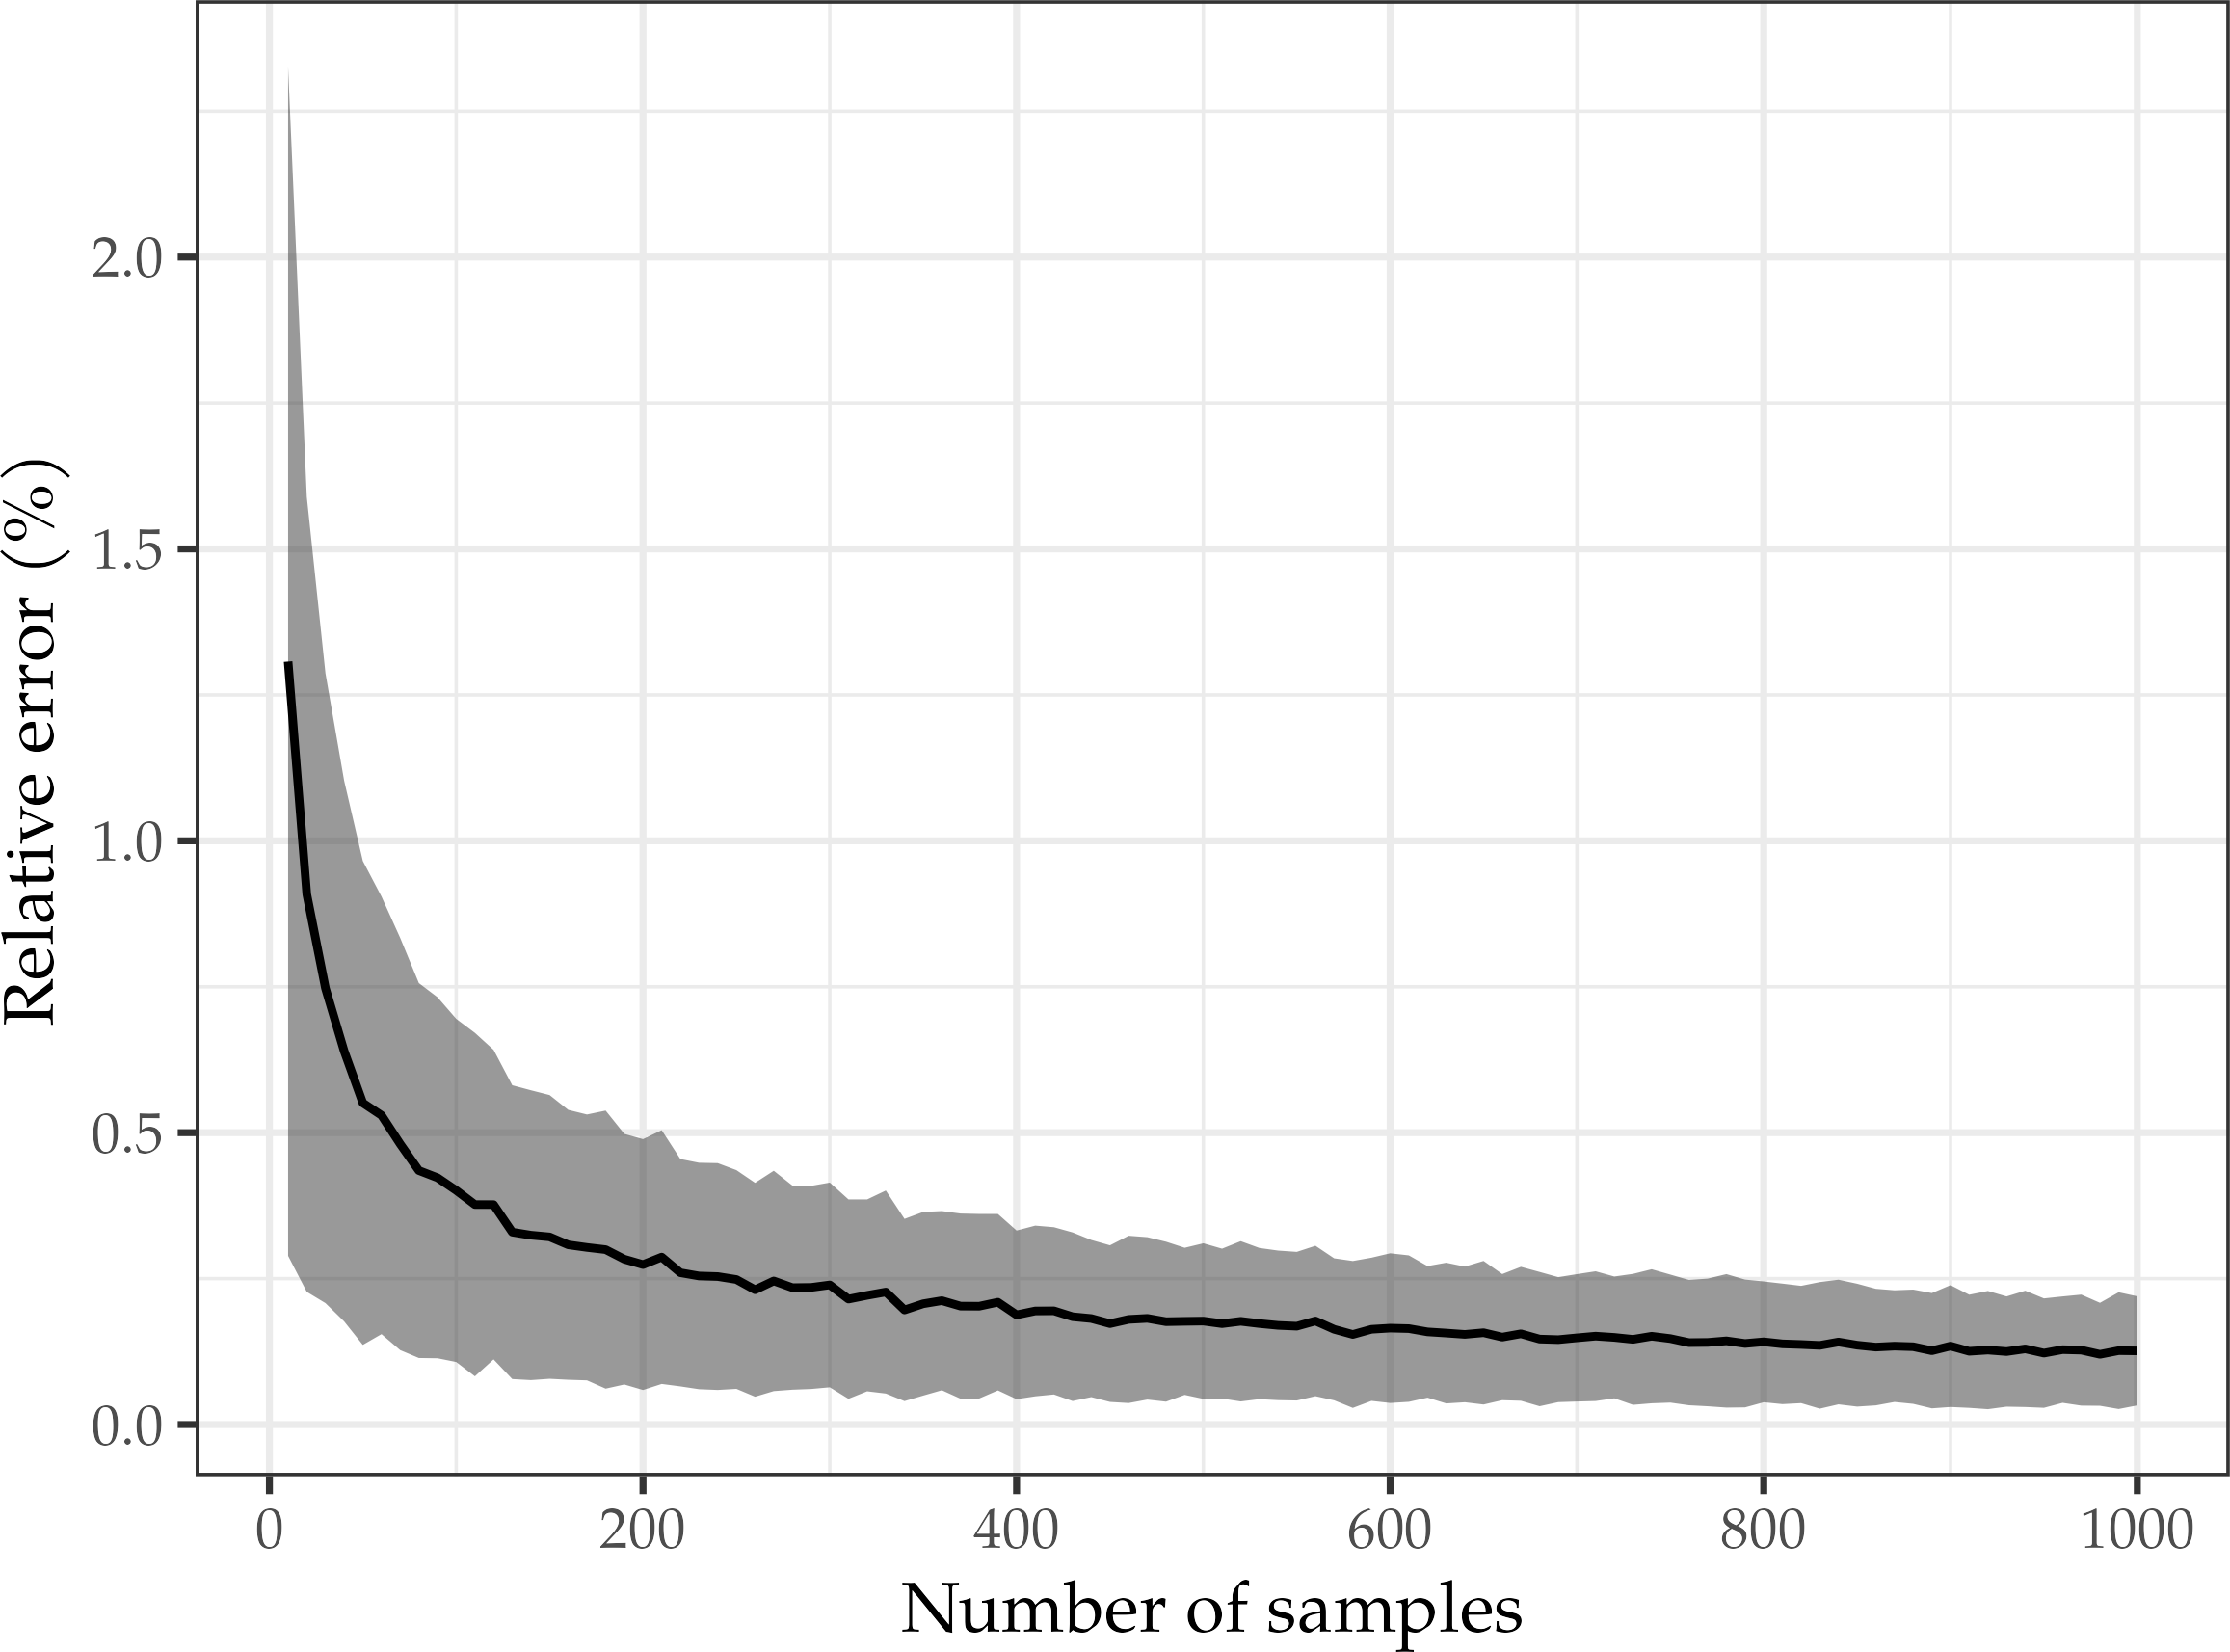
\includegraphics{img/032.png}
  \caption{relative error in the integration of $\cos x$ between $0$ and $\pi/2$
    with the importance sampling technique, as described in \cref{ex:032}. The
    solid lines represent the average over \num{500} realizations, with the
    standard deviation shaded in grey.}
  \label{fig:032}
\end{figure}

\section{Analysing the variance with or without importance sampling}%
\label{ex:033}

\begin{sourcefiles}
  \item[Analysis script] src/033\_variance\_comparison.R
\end{sourcefiles}

This exercise asked to investigate the improvement one can get with importance
sampling applied to a simple integral, the average on the distribution $\rho(x)
= e^{-x}$, $x \geq 0$, of the function
\begin{equation}
  f(x) =
  \begin{cases}
    0 &\quad \text{for } 0 \leq x < T, \\
    1 &\quad \text{for } x \geq T.
  \end{cases}
\end{equation}
This average can be readily calculated as
\begin{equation}
  \expval{f}_{\rho} = \int_{0}^{\infty} f(x) e^{-x} \, dx = \int_{T}^{\infty}
  e^{-x}\, dx = e^{-T}.
\end{equation}
The problem of this integral is that $f(x)$ is different from $0$ in the region
where $\rho(x)$ is quickly vanishing. This means that if we were to sample
numbers from $\rho(x)$ we would waste a lot of iterations.

Consider instead the function $g(x; a) = ae^{-ax}$ defined for $x \geq 0$ and $a
\in (0, 1]$. We can use it for an importance sampling and optimize $a$ to
minimize the variance. In particular, defining $F(x) \coloneq f(x) \rho(x) /
g(x)$ we can write
\begin{equation}
  \expval{f}_{\rho} = \int_{0}^{\infty} f(x) \rho(x) \, dx = 
  \int_{0}^{\infty} \frac{f(x)\rho(x)}{g(x)} g(x) \, dx = 
  \expval{F}_{g}.
\end{equation}
Let’s calculate the second moment now:
\begin{equation}
  \begin{split}
    \expval{F^{2}}_{g} = \int_{0}^{\infty} \frac{f^{2}(x) \rho^2(x)}{g^{2}(x)}
    g(x) \, dx &= \int_{T}^{\infty} \frac{\rho^{2}(x)}{g(x)}\, dx \\
               &= \frac{1}{a} \int_{T}^{\infty} e^{-(2-a) x} \, dx =
               \frac{e^{-(2-a)T}}{a(2-a)}.
  \end{split}
\end{equation}
By subtracting the first moment squared we get the variance,
\begin{equation}
  \sigma^{2}_g(F) = \expval{F^{2}}_g - \expval{F}_{g}^{2}
  = \frac{e^{-(2-a)T}}{a(2-a)} - e^{-2T}.
\end{equation}
The variance of $f$ with respect to $\rho$ is given instead by
\begin{equation}
  \begin{split}
    \sigma^{2}_{\rho}(f)
    = \int_{0}^{\infty} (f(x) - \expval{f}_{\rho})^{2} \rho(x) \, dx
    &= \int_{T}^{\infty} \rho(x) \, dx + \expval{f}_{\rho}^{2}
    - 2 \expval{f}_{\rho} \int_{T}^{\infty} \rho(x) \, dx \\
    &= \expval{f}_{\rho} + \expval{f}^{2}_{\rho} - \expval{f}^{2}_{\rho} \\
    &= e^{-T}(1 - e^{-T}).
  \end{split}
\end{equation}

Now, let’s minimize $\sigma^{2}_g(F)$ with respect to $a$:
\begin{equation}
  \pdiff{}{a} \sigma^{2}_{g}(F) = e^{-(2-a)T} \left[\frac{Ta(2-a) -
  2(1-a)}{a^{2}(2-a)^{2}}\right],
\end{equation}
which gets us to
\begin{equation}
  Ta^{2} - 2(1 + T) a + 2 = 0 \iff a = a^*_{\pm}
  = \frac{1 + T \pm \sqrt{1 + T^{2}}}{T}.
\end{equation}
Only $a^*_{-}$ is compatible with the condition $a \in (0, 1]$, so the optimal
$a$ is given by
\begin{equation}
  a^* = \frac{1 + T - \sqrt{1 + T^{2}}}{T}.
\end{equation}

In \cref{tab:033} I calculated the ratios between each of the two variances and
$\expval{f}_{\rho}$ and the ratio between the two variances, for some values of
$T$. While $\sigma_g(F) / \expval{f}_{\rho}$ grows slowly, $\sigma_\rho(f) /
\expval{f}_{\rho}$ has an exponential increase; indeed
\begin{equation}
  \frac{\sigma_{\rho}(f)}{\expval{f}_{\rho}} = \frac{\sqrt{e^{-T}(1 -
  e^{-T})}}{e^{-T}} = \sqrt{e^{T} - 1}.
\end{equation}
The variance ratio as function of $T$ is also plotted in \cref{fig:033}.

\begin{table}
  \centering
  \captionabove{variance ratios for some values of $T$, all evaluated at
    $a^{*}$.}
  \label{tab:033}
  \begin{tabular}{@{}
      S[table-format=2] S[table-format=5.2, group-separator={}]
      S[table-format=1.2] S[table-format=4.2, group-separator={}]
    @{}}
    \toprule
    {$T$} & {$\sigma_{\rho}(f) / \expval{f}_{\rho}$}
          & {$\sigma_{g}(F) / \expval{F}_{g}$}
          & {$\sigma_{\rho}(f) / \sigma_{g}(F)$} \\
    \midrule
    3  & 4.37  & 1.95 & 2.24 \\
    5  & 12.14 & 2.55 & 4.76 \\
    10 & 148.41 & 3.65 & 40.71 \\
    20 & 22026.47 & 5.18 & 4249.17 \\
    \bottomrule 
  \end{tabular}
\end{table}

\begin{figure}
  \centering
  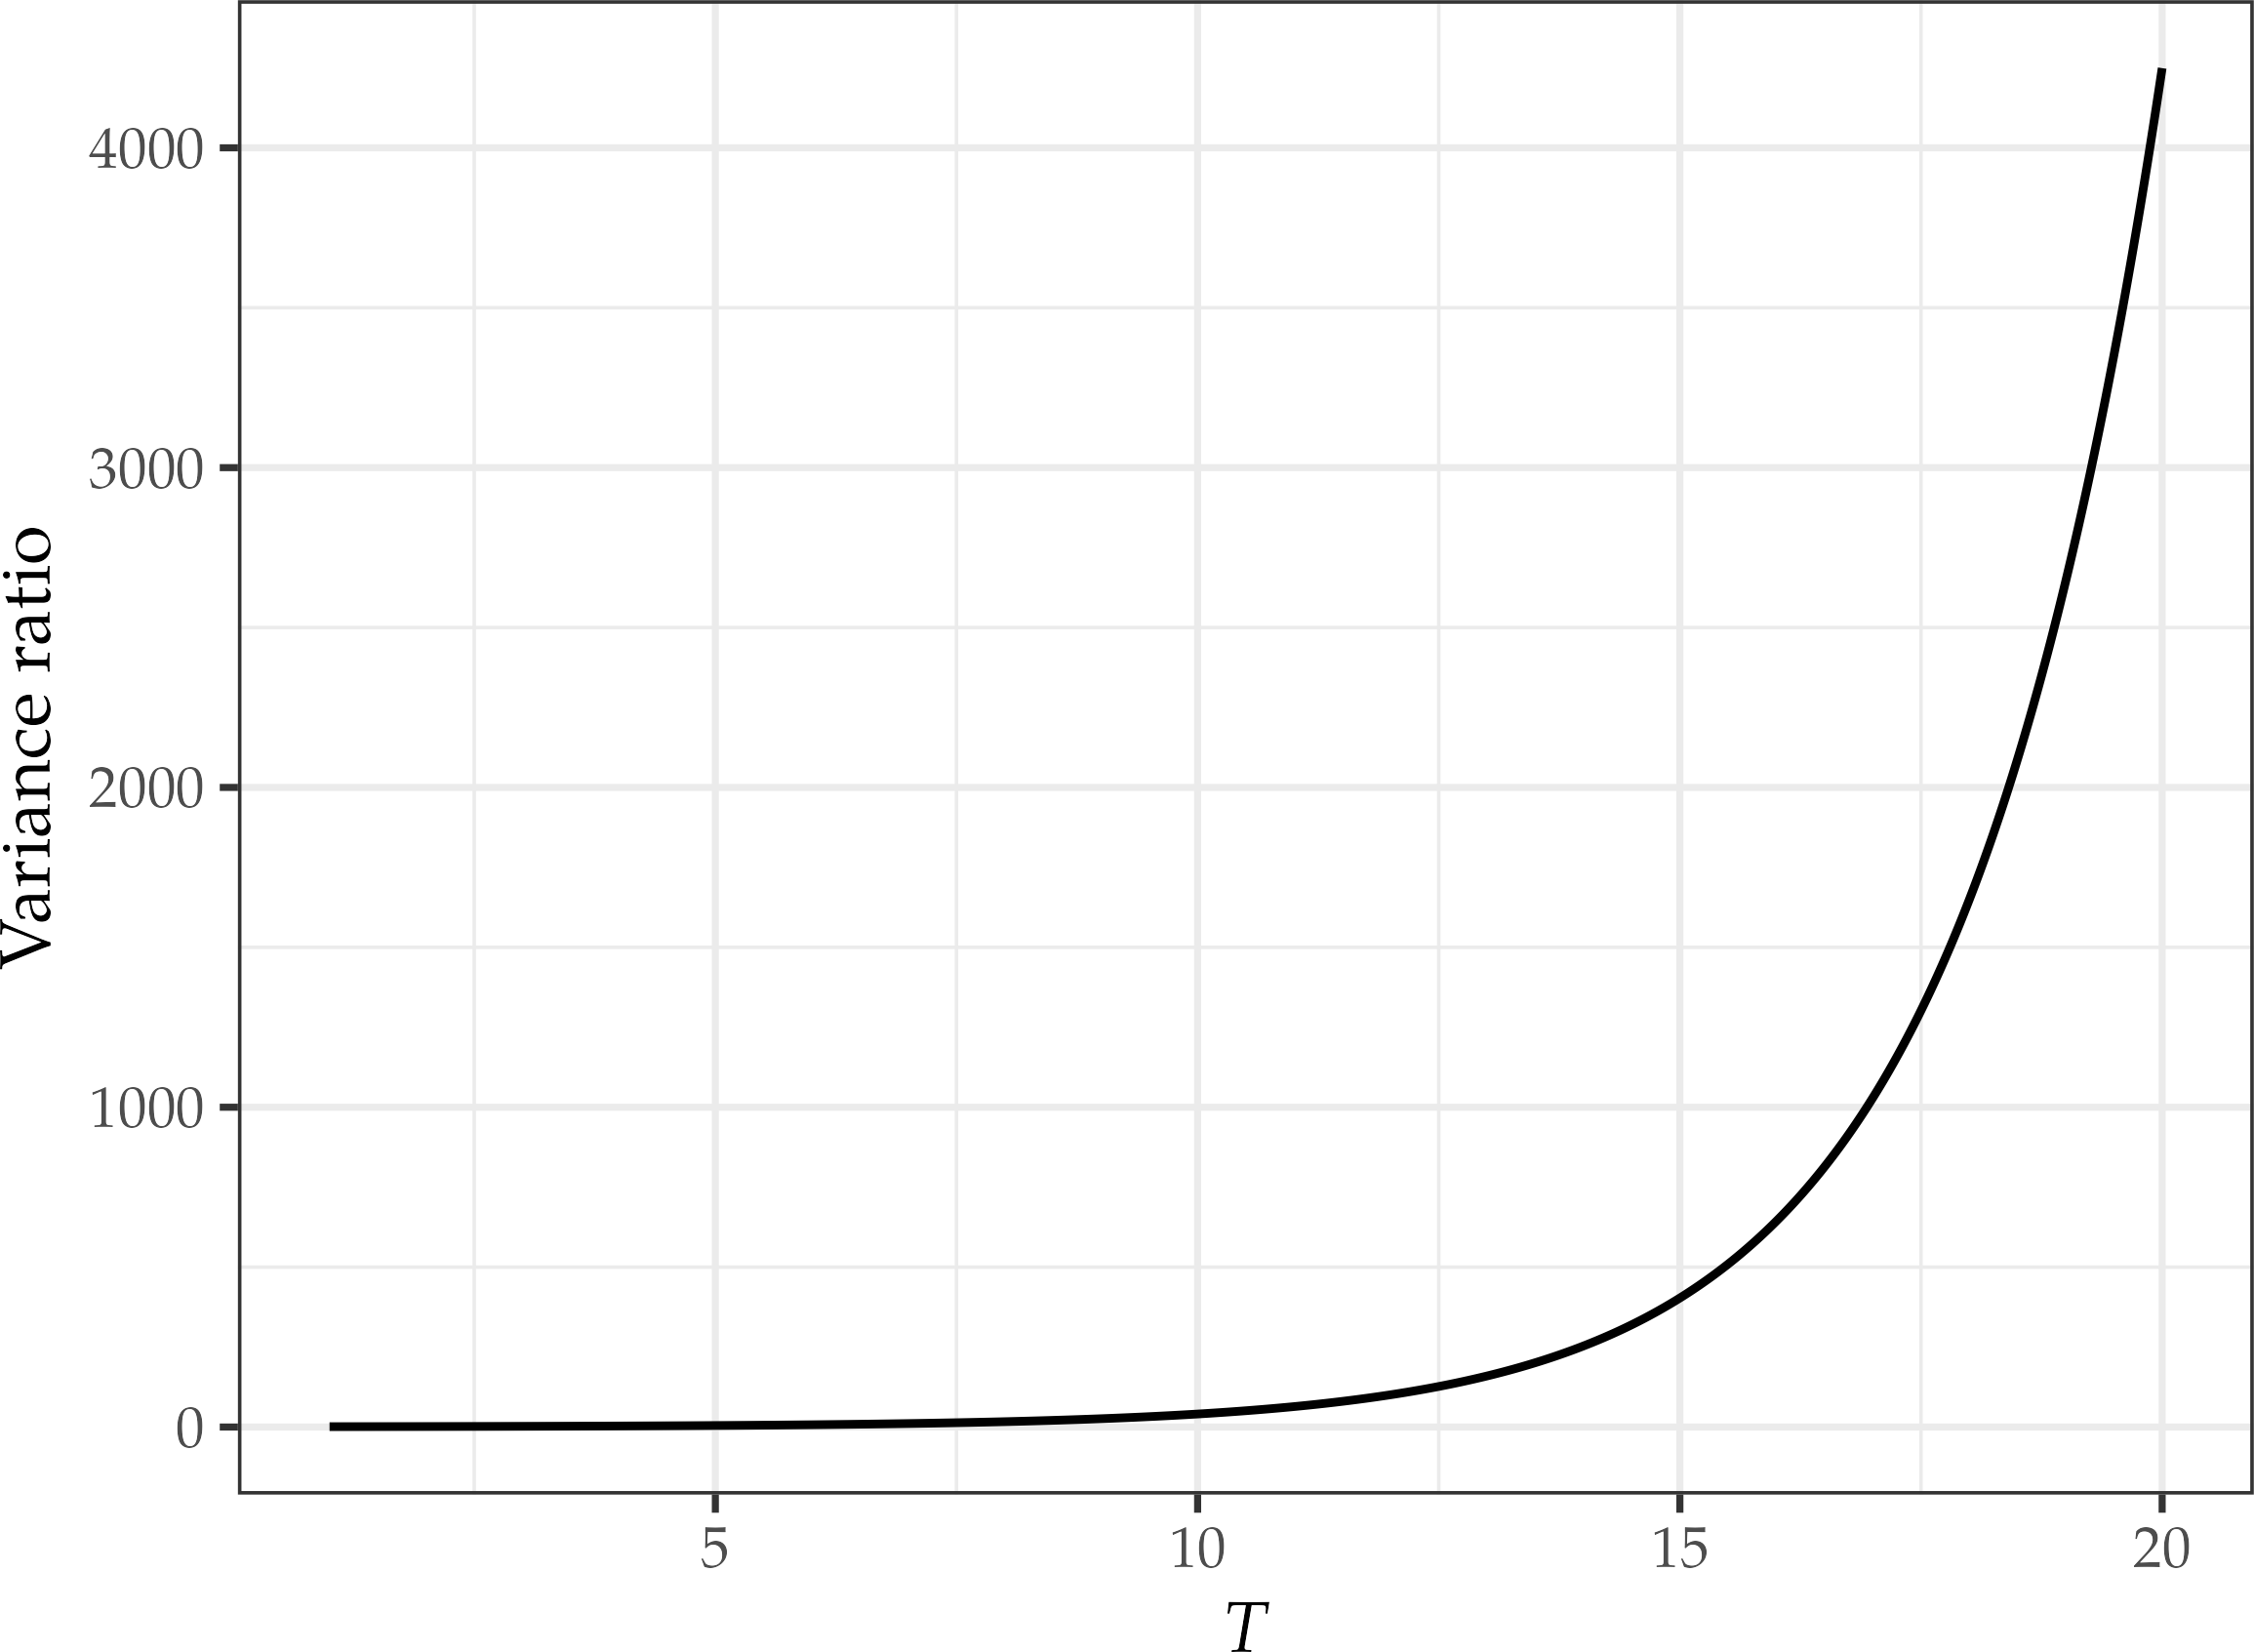
\includegraphics{img/033.png}
  \caption{variance ratio $\frac{\sigma_{\rho}(f)}{\sigma_{g}(F)}$ as a function
    of $T$, from \cref{ex:033}.}
  \label{fig:033}
\end{figure}
